\documentclass[tikz, border=10pt]{standalone}
\usepackage{tikz}
\usetikzlibrary{positioning, arrows.meta, calc, 3d, backgrounds, decorations.pathreplacing, shapes.geometric}

% --- Farben ---
\definecolor{cInput}{RGB}{220, 220, 220} % Grau
\definecolor{cConv}{RGB}{100, 149, 237}  % CornflowerBlue
\definecolor{cPool}{RGB}{255, 127, 80}   % Coral
\definecolor{cDense}{RGB}{144, 238, 144} % LightGreen
\definecolor{cDetail}{RGB}{255, 250, 240} % FloralWhite background

\begin{document}

% Definiere isometrische Projektion
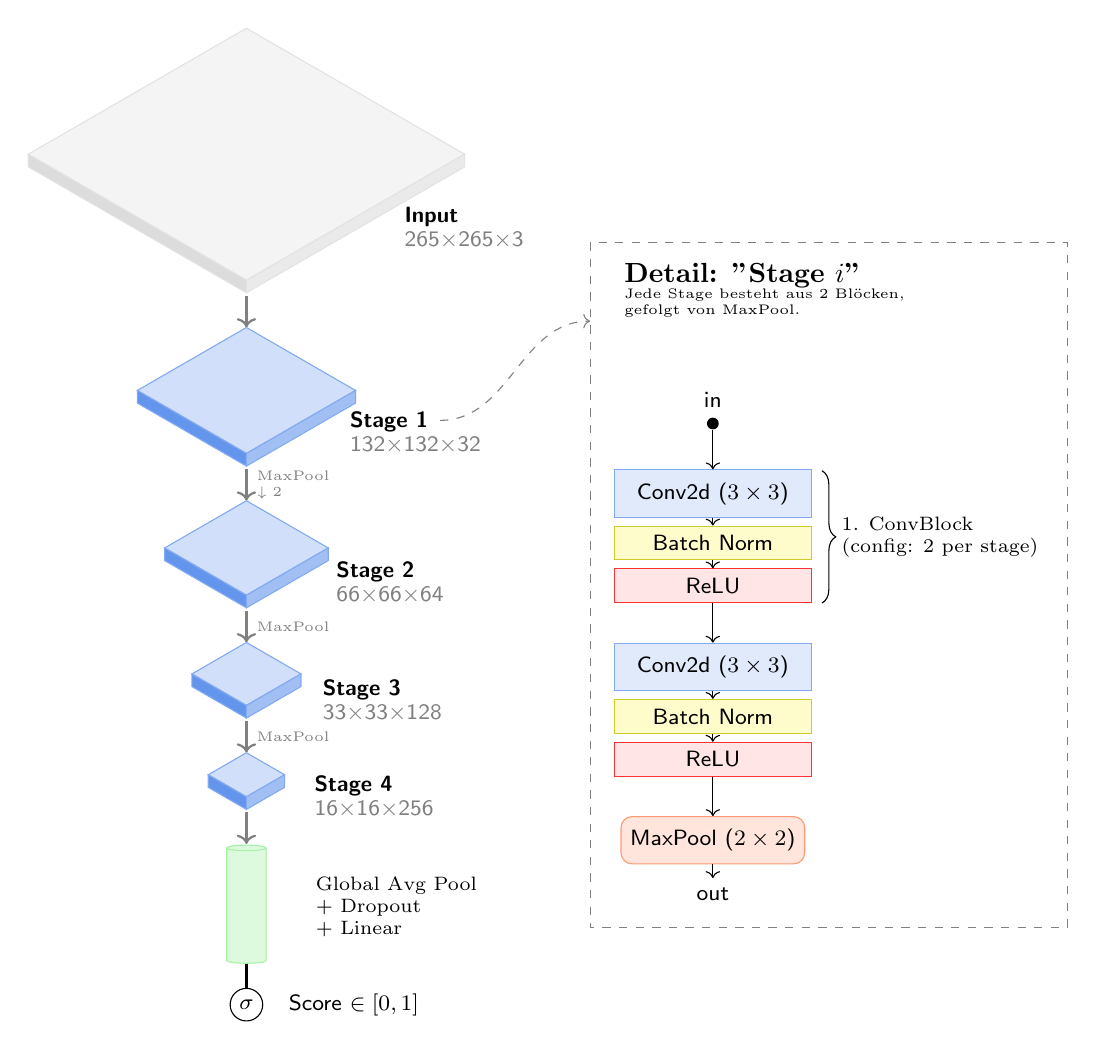
\begin{tikzpicture}[
    x={(0.866cm,-0.5cm)}, 
    y={(0cm,1cm)}, 
    z={(-0.866cm,-0.5cm)},
    scale=0.8,
    font=\sffamily\footnotesize
]

    % --- Makro zum Zeichnen eines 3D-Blocks ---
    \newcommand{\networkLayer}[7]{
        \node (#1_center) #2 {};
        
        \pgfmathsetmacro{\w}{#3/2}
        \pgfmathsetmacro{\d}{#4/2}
        
        \begin{scope}[shift={(#1_center)}]
            % Top Face
            \draw[fill=#5!30, draw=#5!80] (-\w, 0, -\w) -- (\w, 0, -\w) -- (\w, 0, \w) -- (-\w, 0, \w) -- cycle;
            % Front Face
            \draw[fill=#5, draw=#5!80] (-\w, 0, \w) -- (\w, 0, \w) -- (\w, -0.2, \w) -- (-\w, -0.2, \w) -- cycle;
            % Side Face
            \draw[fill=#5!60, draw=#5!80] (\w, 0, \w) -- (\w, 0, -\w) -- (\w, -0.2, -\w) -- (\w, -0.2, \w) -- cycle;
            
            % Beschriftung
            \node[anchor=west, xshift=0.5cm, yshift=-0cm] at (\w, 0, 0) {\textbf{#6}};
            \node[anchor=west, xshift=0.5cm, yshift=-0.3cm, color=gray] at (\w, 0, 0) {#7};
        \end{scope}
    }
    
    % STARTPUNKT OBEN
    \coordinate (current) at (0,0,0);

    % 1. Input Image
    % Position: 0
    \networkLayer{input}{at (current)}{4.0}{0.05}{cInput}{Input}{265$\times$265$\times$3};
    
    % Pfeil runter (Länger gemacht wegen größerem Abstand)
    \draw[->, thick, gray] (0, -2.25, 0) -- (0, -2.75, 0);

    % 2. Stage 1 (Output)
    % Neuer Abstand: -3.5 (vorher -2.5) -> Mehr Platz für den großen Input-Block
    \coordinate (current) at (0, -3.75, 0);
    \networkLayer{stage1}{at (current)}{2.0}{0.3}{cConv}{Stage 1}{132$\times$132$\times$32};
    
    % Pfeil
    \draw[->, thick, gray] (0, -5, 0) -- node[right, font=\tiny, align=left]{MaxPool\\$\downarrow 2$} (0, -5.5, 0);

    % 3. Stage 2 (Output)
    % Neuer Abstand: -7.0 (vorher -5.0) -> Gleichmäßiger
    \coordinate (current) at (0, -6.25, 0);
    \networkLayer{stage2}{at (current)}{1.5}{0.6}{cConv}{Stage 2}{66$\times$66$\times$64};
    
    % Pfeil
    \draw[->, thick, gray] (0, -7.25, 0) -- node[right, font=\tiny]{MaxPool} (0, -7.75, 0);

    % 4. Stage 3 (Output)
    % Neuer Abstand: -10.0 (vorher -7.5/variabel)
    \coordinate (current) at (0, -8.25, 0);
    \networkLayer{stage3}{at (current)}{1.0}{1.0}{cConv}{Stage 3}{33$\times$33$\times$128};
    
    % Pfeil
    \draw[->, thick, gray] (0, -9, 0) -- node[right, font=\tiny]{MaxPool} (0, -9.5, 0);

    % 5. Stage 4 (Output)
    % Neuer Abstand: -12.5
    \coordinate (current) at (0, -9.85, 0);
    \networkLayer{stage4}{at (current)}{0.7}{1.5}{cConv}{Stage 4}{16$\times$16$\times$256};
    
    % Pfeil
    \draw[->, thick, gray] (0, -10.45, 0) -- node[right, font=\tiny]{} (0, -10.95, 0);

    % 6. Head (GAP + FC)
    % Neuer Abstand: -15.0
    \coordinate (gap_pos) at (0, -11.95, 0);
    
    % VERBINDUNG STAGE 4 -> HEAD (Gefixter Pfeil)
    % Wir starten unter Stage 4 und gehen zum Zylinder
    \draw[->, thick, gray] (0, -12, 0) -- (gap_pos);

    % Zylinder zeichnen
    \node (gap) at (gap_pos) [cylinder, shape border rotate=90, draw=cDense!80, fill=cDense!30, minimum height=1.5cm, minimum width=0.5cm, aspect=0.3] {};
    \node[right=0.5cm of gap, font=\scriptsize, align=left] {Global Avg Pool\\+ Dropout\\+ Linear};
    
    % Output
    \coordinate (output_pos) at (0, -13.5, 0);
    \draw[->, thick] (gap.south) -- (output_pos);
    \node (sigmoid) at (output_pos) [circle, draw, fill=white, inner sep=2pt] {$\sigma$};
    \node[right=0.2cm of sigmoid] {Score $\in [0,1]$};


    % --- ZOOM / DETAIL ANSICHT (Rechts) ---
    % Shift erhöht auf x=9.5, damit es nicht überlappt
    \begin{scope}[shift={(8.55, 0)}]
        
        % Rahmen um Detailansicht
        \draw[dashed, gray] (-2.25, 1.75) rectangle (6.5, -4.75);
        \node[anchor=north west, font=\bfseries] at (-1.8, 1.8) {Detail: "Stage $i$"};
        \node[anchor=north west, font=\tiny, text width=4cm] at (-1.8, 1.4) {Jede Stage besteht aus 2 Blöcken, gefolgt von MaxPool.};

        % Verbindungslinie vom Hauptdiagramm (Stage 1) zum Detail
        % Startpunkt angepasst an neue Stage 1 Position
        \draw[dashed, gray, ->] (-5, -2.45) to[out=0, in=180] (-2.25, 0.5);

        % Koordinaten für den internen Fluss
        \node (in) at (0,0) [circle, fill=black, inner sep=1.5pt, label=above:in] {};
        
        % Block 1
        \node (conv1) [draw=cConv!80, fill=cConv!20, rectangle, minimum width=2.5cm, minimum height=0.6cm, below=0.5cm of in] {Conv2d ($3\times3$)};
        \node (bn1) [draw=yellow!80!black, fill=yellow!20, rectangle, minimum width=2.5cm, minimum height=0.4cm, below=0.1cm of conv1] {Batch Norm};
        \node (act1) [draw=red!80, fill=red!10, rectangle, minimum width=2.5cm, minimum height=0.4cm, below=0.1cm of bn1] {ReLU};
        
        % Block 2
        \node (conv2) [draw=cConv!80, fill=cConv!20, rectangle, minimum width=2.5cm, minimum height=0.6cm, below=0.5cm of act1] {Conv2d ($3\times3$)};
        \node (bn2) [draw=yellow!80!black, fill=yellow!20, rectangle, minimum width=2.5cm, minimum height=0.4cm, below=0.1cm of conv2] {Batch Norm};
        \node (act2) [draw=red!80, fill=red!10, rectangle, minimum width=2.5cm, minimum height=0.4cm, below=0.1cm of bn2] {ReLU};

        % MaxPool
        \node (mp) [draw=cPool!80, fill=cPool!20, rectangle, rounded corners, minimum width=2.0cm, minimum height=0.6cm, below=0.5cm of act2] {MaxPool ($2\times2$)};

        % Pfeile Detail
        \draw[->] (in) -- (conv1);
        \draw[->] (conv1) -- (bn1);
        \draw[->] (bn1) -- (act1);
        \draw[->] (act1) -- (conv2);
        \draw[->] (conv2) -- (bn2);
        \draw[->] (bn2) -- (act2);
        \draw[->] (act2) -- (mp);
        \draw[->] (mp) -- +(0,-0.6) node[below] {out};
        
        % Klammer
        \draw[decorate, decoration={brace, amplitude=5pt}] (2, 0.25) -- (2, -1.85) node [midway, xshift=1.5cm, align=left, font=\scriptsize] {1. ConvBlock\\(config: 2 per stage)};
        
    \end{scope}

\end{tikzpicture}
\end{document}